%%%%%%%%%%%%%%%%%%%%%%%%%%%%%%%%%%%%%%%%%%%%%%%%%%%%%
% CHAPTER 4: EXPLORATORY STUDY
%%%%%%%%%%%%%%%%%%%%%%%%%%%%%%%%%%%%%%%%%%%%%%%%%%%%%
%% CONCLUSION
%%%%%%%%%%%%%%%%%%%%%%%%%%%%%%%%%%%%%%%%%%%%%%%%%%%%%
\newpage
\section{Discussion and Conclusion}
\label{exp-study:conclusion}
%%%%%%%%%%%%%%%%%%%%%%%%%%%%%%%%%%%%%%%%%%%%%%%%%%%%%
% EXTRAS FOR CONSIDERATION:
% EXTRA: nature of PIM - see towards a new conceptualization
%%%%%%%%%%%%%%%%%%%%%%%%%%%%%%%%%%%%%%%%%%%%%%%%%%%%%
% * 3 tools/3 ways of working
% * Contrasting user experience
%%%%%%%%%%%%%%%%%%%%%%%%%%%%%%%%%%%%%%%%%%%%%%%%%%%%%
% How to improving PIM experience
% * Most users get by ... are they really that bad?
% * change designs vs. change behaviour
% * Pros and cons of hierarchy. Relate to design rationale in \textbf{Chapter~\ref{chapter:design}}}
%%%%%%%%%%%%%%%%%%%%%%%%%%%%%%%%%%%%%%%%%%%%%%%%%%%%%
% Convergence of PIM tools and other trends
%	* email/bloggers being used to create documents
%	* same interface for multiple types of information (e.g. Windows explorer for docs and bm)
%	* but still sense of distinct collections
%	* Type of integration
%%%%%%%%%%%%%%%%%%%%%%%%%%%%%%%%%%%%%%%%%%%%%%%%%%%%%

%%%%%%%%%%%%%%%%%%%%%%%%
% Recap main findings
%%%%%%%%%%%%%%%%%%%%%%%%
% Recap and discuss substantive findings
% 1.Tool-specific and cross-tool insights
%		e.g. Problems
% 2.Individual differences
% 3.Comparison - Multiple PIM strategies
%		Intra-tool
%		Cross-tool profiling
% 4.Factors affecting PIM strategies
% 5.Conceptual basis
%		Change / time
%		Cross-tool (see below)
% 6.Cross-tool perspective
%		problems
%		activities
% 7.Implications for integration
%		Organizational dimensions
%		Folder Overlap (towards WM)
% 8.Methodological limitations
%	9.Conclusion
%		Moving on

%%%%%%%%%%%%%%%%%%%%%%%%%
% intro & structure
%%%%%%%%%%%%%%%%%%%%%%%%%
% Issues relating to the study methodology are also explored.
This section discusses the chapter's main findings, and relates them to the work presented in subsequent chapters.  Firstly, \textbf{Section~\ref{exp-study:discussion:indiv-diffs}} highlights methodological issues which should be taken into consideration when interpreting the study results. \textbf{Section~\ref{exp-study:discussion:multiple-strategies}} moves on to discuss the observation of multiple organizing strategies, within and across PIM-tools for many participants.  A model is presented to illustrate this new conceptualization of organizing strategies.
% Design implications following from the study findings are discussed. 
\textbf{Section~\ref{exp-study:discussion:integration}} considers implications for the design of PIM-integration technology based on the study findings.
% \textbf{Section~\ref{exp-study:discussion:conceptual-basis}} discusses three properties of PIM as an activity that is: (1) cross-tool, (2) supporting, and (3) ongoing/long-term.
Finally, \textbf{Section~\ref{exp-study:discussion:conclusion}} considers whether the study achieved the objectives in \textbf{Section~\ref{exp-study:introduction}}.



%%%%%%%%%%%%%%%%%%%%%%%%%%%%
% \subsection{Methodological limitations}
%%%%%%%%%%%%%%%%%%%%%%%%%%%%
%%%%%%%%%%%%%%%%%%%%%%%%%%%%%%%%%%%%%%%%%%%%%%%%%%%%%%%%%%%%%%%%%
\subsection{Methodological Limitations}
\label{exp-study:discussion:indiv-diffs}
%%%%%%%%%%%%%%%%%%%%%%%%%%%%%%%%%%%%%%%%%%%%%%%%%%%%%%%%%%%%%%%%%
% Idiosyncratic, individual differences
%%%%%%%%%%%%%%%%%%%%%%%%%%%%%%%%%%%%%
%	\item And also schizophrenic -- The study highlighted the fact that individual users employ a variety/selection of PIM strategies in different parts of the workspace to manage different types of information with varying degrees of success. Most users could not be described as being globally "messy" or "tidy"
%	\item Importance of flexibility. Types of flexibility. Possible concerns for previous technologies - emphasises need for evaluation
%	\item Many key factors affecting choice of PIM strategy (SEE BELOW)
%\end{itemize}
%%%%%%%%%%%%%%%%%%%%%%%%%%%%%%%%%%%%%%%%%%%%%%%%%%%%%%%%%%%%%%%%%
% General METHODOLOGICAL
%%%%%%%%%%%%%%%%%%%%%%%%%%%%%%%%
%The following points are acknowledged regarding validity of results,
%	\item \textit{THINK RELATE TO: methodological discussion in qualitative and quantitative analyses}
%	\item Small sample size. Generally results intended to be indicative, not absolute. 
%	\item Subjectivity of much of the data, tried to balance with objective data
%	\item Limitations of objective data (CAN COVER ABOVE):
%		\item Limitations in collected metadata
%		\item Variations in tools and data collected across individuals
%	\item Limitations of Data Analysis methods (CAN COVER ABOVE)
%		\item Coding scheme, folder overlap (need for IRR?)
%%%%%%%%%%%%%%%%%%%%%%%%%%%%%%%%%%%%%%%%%%%%%%%%%%%%%%%%%%%%%%%%%

The wide range of PIM-related behaviour observed emphasizes the highly individual nature of PIM.  Note that this was the case despite the relatively narrow subject group of technically-experienced, mostly academic participants. It is envisaged that an even wider variety of strategies would be expected in the wider population of computer users. Due to the limited sample size it should be emphasised that the results presented here are intended to be indicative rather than statistically significant across the general user population.
% In fact the one thing that all the participants had in common (and that might generalize universally!) was a general dissatisfaction regarding their PIM tools and the state of their personal information environment (\textit{Subject XYZ: ``there must be a better way of doing it [document management]''}).

%%%%%%%%%%%%%%%%%%%%%%%%%%%%%
% OS AND TOOLS
%%%%%%%%%%%%%%%%%%%%%%%%%%%%%
% Several operating systems were encountered (MacOS, Linux and MS Windows), as well as a wide range of PIM-tools.  
% Variation in practice between operating systems was not considered in the study, due to the small number of participants involved. However it should be noted that all the operating systems were reasonably equivalent in terms of PIM support offered, i.e. hierarchical file system, ability to place of icons on desktop, basic form of email and web browser tools % Relate to BN:95 who tried to compare Win and MacOS operating systems
% Please refer to  \textbf{Table~\ref{table:chapter3_user_summary}} for more detail.
% Secondly, participants also varied in terms of the PIM tools used to manage 
% The tool used to manage document files was typically the graphical file manager provided by default in each operating system (see  \textbf{Table~\ref{table:exp-study:user_summary}}).  \textbf{Table~\ref{table:chapter3_email_and_browser_tools}} shows the range of email tools and web browsers encountered.
It is acknowledged that the study did not control for a number of factors which may influence PIM. Subjects differed both in terms of the operating system used, as well as the specific applications used to manage document files, email and web bookmarks.  Previous studies have noted the variety of tools encountered in studies of email and task management~\citep{Bellotti:00}, and similarly a wide range of PIM tools was observed here.  However, it is argued that most tools were equivalent in terms of functionality offered (hierarchical folder structure, search mechanism etc.). Furthermore, choice of PIM tool did not appear to be a major determinant of PIM strategy, as behaviour varied greatly between  participants using the same tool.  

%%%%%%%%%%%%%%%%%%%%%%%%%%%%%
% FEATURES
%%%%%%%%%%%%%%%%%%%%%%%%%%%%%
% \textit{CITE}), that is containing a wide range of features that can be used in varying ways, or not at all, to the users discretion. \textit{EXPAND}.
Participants also varied in terms of the features used in each tool, and how they used those features. This should not be surprising: PIM tools are complex tools, suffering from ``software bloat''~\citep{mcgrenere:02}.  There is clearly scope for more systematic studies focusing on different aspects of PIM interfaces in specific implementations.  % However, the aim of this study was to gain a broad picture of participants' PIM practices.



%%%%%%%%%%%%%%%%%%%%%%%%%%%%%%%%%%%%%%%%%%%%%%%%%%%%%%%%%%%%%%%%%%%%%%%%%%%%%%%%%%%%%%%%%%%%%%%%%%%%%%%%%%%%%%%%%
%%%%%%%%%%%%%%%%%%%%%%%%%%%%%%%%%%%%%%%%%%%%%%%%%%%%%%%%%%%%%%%%%%%%%%%%%%%%%%%%%%%%%%%%%%%%%%%%%%%%%%%%%%%%%%%%%
%%%%%%%%%%%%%%%%%%%%%%%%%%%%%%%%%%%%%%%%%%%%%%%%%%%%%%%%%%%%%%%%%%%%%%%%%%%%%%%%%%%%%%%%%%%%%%%%%%%%%%%%%%%%%%%%%
%%%%%%%%%%%%%%%%%%%%%%%%%%%%%%%%%%%%%%%%%%%%%%%%%%%%%%%%%%%%%%%%%%%%%%%%%%%%%%%%%%%%%%%%%%%%%%%%%%%%%%%%%%%%%%%%%

%%%%%%%%%%%%%%%%%%%%%%%%%%%%%%%%%%%%%%
\subsection{Multiple Organizing Strategies}
\label{exp-study:discussion:multiple-strategies}
%%%%%%%%%%%%%%%%%%%%%%%%%%%%%%%%%%%%%%
%\textit {Relate to Barreau: indicated that ``users employed different classifying rules based upon level of granularity required to support the workload''}. MOVE TO ORG?
%%%%%%%%%%%%%%%%%%%%%%%%%%%%%%%%%%%%%%%%%%%%%%%%%%%%%%%%%%%%%%%%%%%%%%%%%%%%%%%%%%
%	\item employ different strategies within a particular PIM tool
%	\item across different PIM tools for managing the same type of information
%	\item across different PIM tools for managing different types of information
%	\item and that's before WE then consider extended personal workspace.
%%%%%%%%%%%%%%%%%%%%%%%%%%%%%%%%%%%%%%%%%%%%%%%%%%%%%%%%%%%%%%%%%%%%%%%%%%%%%%%%%%

%%%%%%%%%%%%%%%%%%%%%%%%%%%%%%%%%%
% MOVE THE FOLLOWING TO CHAPTER 4
% DISCUSS RESULT
%%%%%%%%%%%%%%%%%%%%%%%%%%%%%%%%%%
%Users are not ``messies'' OR ``tidies'' -- they tend to be a bit of both, depends on where you're looking.  Previous classifications have represented users as extreme charactitures.
% {DISCUSS: Develop messy/tidy theme - is messy good?  What is messy? Drag in Mr. Men and that Economist article}
% Key factors contributing to variation are identified
% A number of factors contributing to the variation in strategy across different types of personal information were identified in \textbf{Section~\ref{exp-study:conclusion}}.

%%%%%%%%%%%%%%%%%%%%%%%%%%%%%%%%%%%%%%%%%%%%%%%%
% Use of ``multi strats'' findings in rest of chapter/ thesis
%%%%%%%%%%%%%%%%%%%%%%%%%%%%%%%%%%%%%%%%%%%%%%%%
%The findings regarding multiple strategies are used in a number of ways in this chapter:
%\begin{enumerate}
%\item To explain the change behaviour observed  below -- and to motivate theory of changes in \textbf{Section~\ref{disc:theory-discussion}}.
%\item Use to explain WM evaluation results in terms of partial WM uptake \textbf{Section~\ref{disc:evaluation-discussion}}.
%\item Used to make design recommendations in \textbf{Section~\ref{disc:design-guidelines-discussion}}.
%\end{enumerate}

\textbf{Section~\ref{exp-study:Results-org-strategies}} highlighted that not only are organizing strategies highly idiosyncratic (varying between users), but they also vary \textit{within and between tools for specific user}. As far as the author is aware, this is the first study to systematically investigate the variety of PIM strategies employed by an individual across a range of tools.  

% it also observed a wide variety of strategies employed in different tools  % These two degrees of variance in terms of PIM strategy are referred to here as (1) \textit{idiosyncratic} (variance between users) and (2) \textit{schizophrenic} (variance between tools for the same user).

Previous studies have noted variation in organizing strategies between users for a specific tool.  However, the findings presented in \textbf{Section~\ref{exp-study:Results-org-strategies}} suggest that much user behaviour does not map onto strategy classifications that have been offered in email and bookmarks~\citep{da:98,ob:97,Whittaker-email:96}. Although such classifications offer useful abstractions of PIM practice, the author contends that they exaggerate the extremes -- portraying users as either \textit{messy} or \textit{tidy}, \textit{filers} or \textit{no-filers}. \textbf{Section~\ref{exp-study:Results-org-strategies}} attempts to classify behaviour in more detail to take account of multiple strategies.  Previous work has also noted multiple strategies in the context of paper archives, where people tend to combine filing and piling strategies~\citep{Whittaker-paper:01}. 

% Many participants employed multiple PIM strategies within specific collections.
The cross-tool data indicates that PIM strategies also vary significantly \textit{between} tools for many individuals. Previous work has not taken such cross-tool variation into account.  The results presented in \textbf{Section~\ref{exp-study:Results-org-strategies}} focus on variations in organizing strategy, e.g. participants tended to organize files more extensively than emails or bookmarks.  In other words, one can not assume that a frequent filer in email is necessarily tidy everywhere.
The following factors may contribute towards variation in organizing strategy:
\begin{itemize}
%* Value of information, relative to perceived overheads
\item \textit{The perceived value of information} -- Users feel a strong sense of ownership over files, which they have often invested significant time in authoring, and are therefore willing to take the time to organize. In contrast they feel less ownership over email and the websites referred to by bookmarks, which are typically authored by other users.

%* Other PIM strategies/retrieval factors
\item \textit{Likelihood and style of retrieval} -- The study data suggests that users are more likely to re-use files than emails or bookmarks, particularly over the long-term. Users perceive that file organization is more worthwhile since the cost of filing is offset by predicted benefits at retrieval time. Also, users tend to retrieve email by sorting on metadata, such as "sender" and "date received". Therefore there is less need to organize to facilitate folder-based browsing.

%* Other PIM strategies/acquisition factors
\item \textit{Acquisition-related factors} -- Files and bookmarks are created incrementally, making them easier to organize than email, which is acquired in an uncontrolled way. Many users who would like to organize their email do not have time to do so due to the high number of messages~\citep{Whittaker-email:96}.

\item \textit{Attitude towards organizing} -- As well as the nature of information managed in each tool, the data suggests that a user's tendency to organize may be influenced by personality factors. Participants who stated that being tidy was important tended to be consistently pro-organizing in multiple tools.

%%%%%%%%%%%%%%%%%%%%%%%%%%
% Environmental factors
%%%%%%%%%%%%%%%%%%%%%%%%%%
% Social context - (e.g. social exposure, office procedures). Trying to impress people (ref; Gosling))
% Technological context - (e.g. space)
% Work context - Demands of production task

\end{itemize}

%%%%%%%%%%%%%%%%%%%%%%%%%%%%%%%%%%%%%%
\subsubsection{Model of Multiple Organizing Strategies}
\label{exp-study:multiple-strategies-model}
%%%%%%%%%%%%%%%%%%%%%%%%%%%%%%%%%%%%%%
%%%%%%%%%%%%%%%%%%%%%%%%%%%%%%%%%
% Activities vary across tools
%%%%%%%%%%%%%%%%%%%%%%%%%%%%%%%%%
% Building on the model presented in \textbf{Section~\ref{discussion:cross-tool:activity-model}}, a model of PIM strategies is proposed to reflect the empirical findings reported in \textbf{Chapters~\ref{chapter:exploratory_study}} and \textbf{\ref{chapter:main-study}}.  Finally, implications for design and methodology are discussed.
% One user -- different strategies in each tool. The study highlighted the fact that individual users employ a variety/selection of PIM strategies in different parts of the workspace to manage different types of information with varying degrees of success. Tool form very similar but contexts of use very different
%%%%%%%%%%%%%%%%%%%%%%%%%%%%%%%%%%%%%%%%%%%%%%
% \subsection{A cross-tool strategy view}
% \label{discussion:strategies-cross-tool}
%%%%%%%%%%%%%%%%%%%%%%%%%%%%%%%%%%%%%%%%%%%%%%
% This section offers a new conceptualization of PIM strategies.  Firstly, a descriptive model of PIM strategy is developed, encompassing the observations of multiple strategies in both tool-specific and cross-tool contexts.
% A framework for conceptualizing PIM strategies is proposed as follows.
A new conceptualization of organizing strategies is suggested by the findings in \textbf{Section~\ref{exp-study:Results-org-strategies}}. 
% Following from the cross-tool perspective, a cross-tool conceptualization of PIM strategies can be outlined. The model is illustrated diagrammatically in  and described as follows: 
\textbf{Figure ~\ref{fig:discussion:PIM-cross-tool-strategies}} illustrates three levels at which strategies can be described:
\begin{enumerate}

%%%%%%%%%%%%%%%%%%%%%%%%%
% Information-level
%%%%%%%%%%%%%%%%%%%%%%%%%
\item \textit{Item-level} -- Within the boundaries of a particular PIM-tool, a user may employ various organizing strategies for different items.  For example, within an email collection, those messages relating to a particular project may be carefully filed in a dedicated folder, whilst other messages may be left in the inbox.

%%%%%%%%%%%%%%%%%%%%%%%%%
% Tool-level
%%%%%%%%%%%%%%%%%%%%%%%%%
\item \textit{Tool-level} -- Within a single tool context containing many types of items, a user may employ \textit{multiple organizing strategies}, e.g. 20\% frequent filer, and 80\% spring-cleaner.  \textbf{Chapter~\ref{chapter:main-study}} builds on this conceptualization of multiple strategies to model the incremental nature of changes in organizing strategy.

These multiple strategies may be combined as a reflection of the user's overall ``trait'', such as the proposed \textit{pro-organizing} and \textit{organizing-neutral}.  An outside observer glancing at a user's PIM-tool would build up an impression of their PIM strategies at this level, for example as ``messy'' (organizing-neutral), or ``tidy'' (pro-organizing).  % These two extremes correspond to the no-filer and frequent-filer profiles from~\citet{Whittaker-email:96}
% \textbf{Chapter~\ref{chapter:exploratory_study}} noted the \textit{multiple-strategies} employed by users within specific collections of personal information, and also across different collections.  Previous strategy classifications were criticised for not reflecting this low-level detail.
However, such traits abstract much low-level detail.  For example an apparently ``messy'' email user may be highly organized with respect to certain types of email.  Previous classifications of organizing behaviour have been shown to be limited in this way.  % 

%%%%%%%%%%%%%%%%%%%%%%%%%
% CROSS-Tool-level
%%%%%%%%%%%%%%%%%%%%%%%%%
% \item Cross-tool: tool-specific traits, contributing to overall trait
% % Likewise the tool-specific traits can combine to give an overall trait, as in the cross-tool profile presented.
\item \textit{Cross-tool level} -- At the level of the entire computer, tool-specific strategies can be aggregated to form a ``cross-tool trait'', as with the cross-tool profile in \textbf{Section~\ref{exp-study:Results-cross-tool-profiling}}.  Again, it is noted that a focus at this high a level again abstracts much lower-level behaviour.
\end{enumerate}

% %%%%%%%%%%%%%%%%%%%%%%%%%%%%%
% FIGURE - Cross-tool strategy model
% %%%%%%%%%%%%%%%%%%%%%%%%%%%%%
%%%%%%%%%%%%%%%%%%%%%%%%%%%%%%
\begin{figure}[hbtp]
	\begin{center}
		\leavevmode
		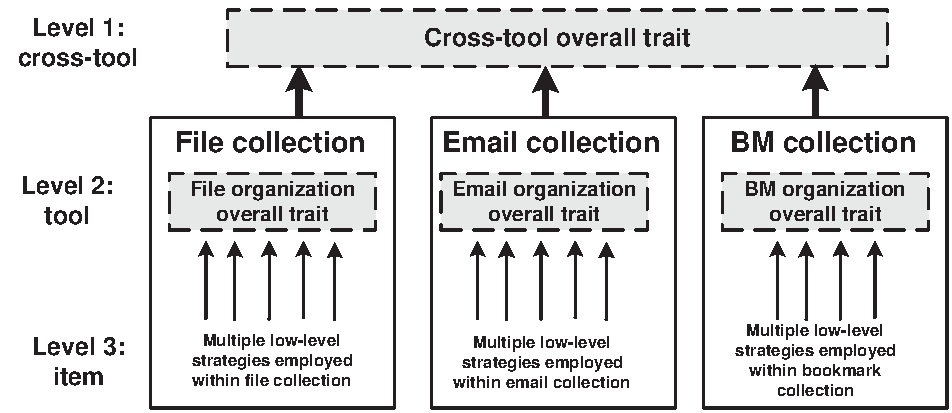
\includegraphics[height=5cm]{pictures/exp-study/PIM-cross-tool-strategies.pdf}
		% fs-fm-comparison.pdf}
	\end{center}
	\caption{Three-level model of an individual's organizing strategies}
	\label{fig:discussion:PIM-cross-tool-strategies}
\end{figure}

% The findings from this study show that you cannot generalize from one level to another. 
This conceptualization emphasises the importance of specifying the level of analysis when talking about phenomena such as organizing strategies.



%%%%%%%%%%%%%%%%%%%%%%%%%%%%%%%%%%%%%%%%%%%%%%%%%%%%%%%%%%%%
% \textit{Include stuff regarding how to talk about strategies}
%%%%%%%%%%%%%%%%%%%%%%%%%%%%%%%%%%%%%%%%%%%%%%%%%%%%%%%%%%%%

%%%%%%%%%%%%%%%%%%%%%%%%%%%%%%%%%%%%%%%%%%%%%%%%%%%%%%%%%%%%%%%%%%%%%%%%%%%%%%%%%%%%%%%%%%%%%%%%%%%%%%%%%%%%%%%%%
%%%%%%%%%%%%%%%%%%%%%%%%%%%%%%%%%%%%%%%%%%%%%%%%%%%%%%%%%%%%%%%%%%%%%%%%%%%%%%%%%%%%%%%%%%%%%%%%%%%%%%%%%%%%%%%%%
%%%%%%%%%%%%%%%%%%%%%%%%%%%%%%%%%%%%%%%%%%%%%%%%%%%%%%%%%%%%%%%%%%%%%%%%%%%%%%%%%%%%%%%%%%%%%%%%%%%%%%%%%%%%%%%%%
%%%%%%%%%%%%%%%%%%%%%%%%%%%%%%%%%%%%%%%%%%%%%%%%%%%%%%%%%%%%%%%%%%%%%%%%%%%%%%%%%%%%%%%%%%%%%%%%%%%%%%%%%%%%%%%%%

%%%%%%%%%%%%%%%%%%%%%%%%%%%%%%%%%%%%%%%%%%
\subsection{Implications for Design}
\label{exp-study:discussion:integration}
%%%%%%%%%%%%%%%%%%%%%%%%%%%%%%%%%%%%%%%%%%

Integration between PIM-tools has been repeatedly put forward as a worthy design aim~\citep{Bellotti:03,Bergman:03,rpb:01a,Dumais:03a,Kaptelinin:03}, but with little empirical support.  It is argued that cross-tool studies such as this one can provide an empirical foundation for such design by highlighting: (1) synergies between tools that can be exploited to improve integration, and (2) differences between tool usage that may indicate barriers to integration.
%%%%%%%%%%%%%%
% PROBLEMS
%%%%%%%%%%%%%%
% In particular, our research is concerned with the problems users encounter across multiple tools whilst performing two PIM-related activities: 1.	Folder organization - the management of items within a folder hierarchy made up of user-defined categories 2.	Reminder Management - the use of items as implicit reminders (or "to-do" items)}
%		Provision of insights into possible upsides and downsides of integration/unification. ID of key issues. See below
\textbf{Section~\ref{exp-study:comparison-problems}} highlighted a number of problems that either, (a) occur in multiple tool contexts, or (b) bridge multiple tools.  The first type of problem can potentially be solved by a cross-tool design strategy, where the same improvement is made to multiple tools.  The second type of problem confirms the potential of improving integration between PIM-tools. Other findings from the study indicate possible routes for integration. % may suggest appropriate routes for cross-tool integration (see \textbf{Section~\ref{exp-study:discussion:integration}}).  % \textbf{Chapter~\ref{chapter:design}} reports the design of a cross-tool integration mechanism. 

%%%%%%%%%%%%%%%%%%%%%%%%%%%%%%%%%%%%%%%
% Link from folder overlap towards WorkspaceMirror}
%%%%%%%%%%%%%%%%%%%%%%%%%%%%%%%%%%%%%%%
% Ideas generated for cross-tool design work later in thesis are summarized.
% \textit{Folder overlap} suggests a mismatch between the production activities (involving multiple PIM tools) and tool-centric PIM support. 
The observation of \textit{folder overlap} in \textbf{Section~\ref{exp-study:Results-folder-overlap}} points to a subset of user activities that involve the management of multiple types of information.  Most overlapping folders corresponded to \textit{roles} and \textit{projects}, suggesting that these concepts may be usefully shared between collections, as in UMEA~\citep{Kaptelinin:03}. However, it should be emphasized that most folders did not overlap. This suggests that: (1) some production tasks are supported by single PIM tools and may not necessarily benefit from increased integration; and (2) users may have different organizational needs in different tools.  Folder overlap forms the empirical basis for the integration technology developed in \textbf{Chapter~\ref{chapter:design}}.

The author notes the potential compatibility for integration of files and \textit{filed} email. Both types of information are either self-created or assessed as having long-term value.  Also, folder overlap was greatest between these collections.  However, complete unification between files and all email (as pointed to by designs such as TaskMaster~\citep{Bellotti:03}) may lead to the disruption of more controlled items (e.g. files, tasks) by unprocessed email. In some cases it may be appropriate not to integrate - but to instead retain separation between tools.  This measured view of the pros and cons of integration is developed further in \textbf{Chapter~\ref{chapter:discussion}}.

The investigation of \textit{organizational dimensions} in \textbf{Section~\ref{exp-study:Results-org-dims}} points to users having different organizational needs in different tool contexts.  It indicates that email contains more \textit{contact}-based folders, whilst bookmark folders are mainly \textit{interest}-based.  This variety suggests users may be constrained by any PIM-tools that are based on specific types of concept. An example in the PIM-integration genre is UMEA~\citep{Kaptelinin:03}, which focuses on \textit{projects}. 

Finally, the discussion in \textbf{Section~\ref{exp-study:discussion:multiple-strategies}} underlines the challenge of PIM design.  Designers must not only cater for individual differences between users, but also for an individual user's \textit{multiple strategies}.  Future design must take account of strategy variation by providing the flexibility to manage different types of information in distinct ways -- both within a single collection, and across collections. For instance, tools should allow users to different items as required, whilst not penalizing those users who do not want to organize. 


% In our future work WE plan to consider integration with other PIM tools (e.g. calendars), and devices involved in PIM (e.g. PDA devices).

%%%%%%%%%%%%%%%%%%%%%%%%%%
% CUE NEED TO EVALUATE
%%%%%%%%%%%%%%%%%%%%%%%%%%


%%%%%%%%%%%%%%%%%%%%%%%%%%%%%%%%%%%%%%%%%%%%%%%%%%%%%%%%%%%%%%%%%%%%%%%%%%%%%%%%%%%%%%%%%%%%%%%%%%%%%%%%%%%%%%%%%
%%%%%%%%%%%%%%%%%%%%%%%%%%%%%%%%%%%%%%%%%%%%%%%%%%%%%%%%%%%%%%%%%%%%%%%%%%%%%%%%%%%%%%%%%%%%%%%%%%%%%%%%%%%%%%%%%
%%%%%%%%%%%%%%%%%%%%%%%%%%%%%%%%%%%%%%%%%%%%%%%%%%%%%%%%%%%%%%%%%%%%%%%%%%%%%%%%%%%%%%%%%%%%%%%%%%%%%%%%%%%%%%%%%
%%%%%%%%%%%%%%%%%%%%%%%%%%%%%%%%%%%%%%%%%%%%%%%%%%%%%%%%%%%%%%%%%%%%%%%%%%%%%%%%%%%%%%%%%%%%%%%%%%%%%%%%%%%%%%%%%

%%%%%%%%%%%%%%%%%%%%%%%%%%%%%%%%%%%%%%%%%%%%%%%%%%%%
%\subsection{Refining the conceptual basis of PIM}
%\label{exp-study:discussion:conceptual-basis}
%%%%%%%%%%%%%%%%%%%%%%%%%%%%%%%%%%%%%%%%%%%%%%%%%%%%
% Other aspects of pim to consider as follows
%%%%%%%%%%%%%%%%%%%%%%%%%%%%%%%%%%%%%%%%%%%%%%%%%%%%
% COMPLEX/DIFFICULT
%%%%%%%%%%%%%%%%%%%%%%%%%%%
%	\item TO PLACE: ANXIETY OF ORDER: even relatively organised users considered themselves messy (i.e. not dictated by number of folders present, as can be failed folders)
%%%%%%%%%%%%%%%%%%%%%%%%%%%%%%%%%%%%%%%%%%%%%%%%%%%%
% Satisficing nature}
%%%%%%%%%%%%%%%%%%%%%%%%%%%
%	\item Organization, maintenance \textit{QUOTE: "`better things to do"'}
%	\item Idiosyncratic cost/benefit trade-off's
%%%%%%%%%%%%%%%%%%%%%%%%%%%%%%%%%%%%%%%%%%%%%%%%%%%%

%The study findings highlight several properties of PIM to be developed in subsequent chapters:
% Insights provided by the study indicate several directions for improving the current conceptual basis for PIM.  
%\begin{itemize}

%%%%%%%%%%%%%%%%%%%%%%%%%%%%%%%%%%%%%%%%%%%%%%%
% CROSS-TOOL NATURE - discussed in more detail below
%		\textbf{Towards a Cross-tool Perspective} -- a different way of looking at the problem.
%		Move from typical tool-centric towards cross-tool view.
%		Inter-relationship between tools is key.
%%%%%%%%%%%%%%%%%%%%%%%%%%%%%%%%%%%%%%%%%%%%%%%
% \subsubsection{PIM as a cross-tool activity}
%%%%%%%%%%%%%%%%%%%%%%%%%%%%%%%%%%%%%%%%%%%%%%%
% \item \textit{PIM as a cross-tool activity} --  Firstly, the study highlighted the cross-tool nature of PIM. Barreau conceptualized the computer as a single abstract PIM system, whereas from a cross-tool perspective it is clear that current PIM-tools constitute a set of parallel yet inter-related systems, in which different types of information are managed in different ways.   This is despite the fact that the different tools are similar in form (e.g. folder-based organizing mechanism).

%%%%%%%%%%%%%%%%%%%%%%%%%%%%%%
% Activities are cross-tool
%%%%%%%%%%%%%%%%%%%%%%%%%%%%%%
% Introduce link to cross-tool abstractions of PIM, e.g. IM and TM. LINK to discussion. \textit{Relate to similar design/theoretical perspectives, e.g. Raskin, Kirsh, Kaptelinin}
% \textbf{Section~\ref{exp-study:comparison-problems}} provided a range of evidence that many PIM-related problems are cross-tool. Aspects of PIM such as information management and task management can be considered as cross-tool: they cut across a wide range of tools.

% OTHER DEVICES
% Note that the study only considered the desktop workspace. One can of course consider PIM across the various computers and mobile devices used by an individual
%	DISCUSS: Relate to beyond the scope of this study (i.e. beyond desktop) as well. Also consider physical comparison, and different physical locations (\textit{QUOTES: bob, sil})


%%%%%%%%%%%%%%%%%%%%%%%%%%%%%%%%%%%%%%%%%%%%%%%%%%%%%
% PIM as a SUPPORTING activity
%%%%%%%%%%%%%%%%%%%%%%%%%%%%%%%%%%%%%%%%%%%%%%%
% \textbf{Section~\ref{exp-study:Results-folder-overlap}} discussed the observation of folder overlap -- folders which existed in multiple PIM-tool contexts. Overlapping folders are interpreted as an indication of production activities that involve the management of multiple types of personal information.
% \item \textit{PIM as a supporting activity} -- \textbf{Chapter~\ref{chapter:discussion}} discusses the view that PIM is a supporting activity.  Some key evidence for this view was uncovered in this study.  Firstly, \textbf{Section~\ref{exp-study:comparison-changes}} observed that the study had a strong ``auditing'' effect on user behaviour, making them think more about PIM than they normally would. %textbf{Section~\ref{exp-study:Results-folder-overlap}} discussed the concept of folder overlap -- folders which existed in multiple PIM-tool contexts.  Overlapping folders are interpreted as an indication of production activities that involve the management of multiple types of personal information.




%%%%%%%%%%%%%%%%%%%%%%%%%%%%%%%%%%%%%%%%%%%%%%%%%%%%%
% PIM as an ONGOING background activity
%%%%%%%%%%%%%%%%%%%%%%%%%%%%%%%%%%%%%%%%%%%%%%%
%\textbf{NEW: pressure/complexity/stress/never-ending}
%\item \textit{PIM as an ongoing activity} -- Although the study was non-longitudinal, some insights into the evolving nature of PIM behaviour were revealed.  In particular, \textbf{Section~\ref{exp-study:comparison-changes}} described participants reports of `historical changes in organizing strategy, including both increases and decreases in filing tendency. These observations partially motivated the longitudinal PIM study reported in \textbf{Chapter~\ref{chapter:main-study}}.

%\end{itemize}

%%%%%%%%%%%%%%%%%%%%%%%%%%%%%%%
% THEORY-BUILDING; CHAPTER 7
%%%%%%%%%%%%%%%%%%%%%%%%%%%%%%%
% WE are continuing our data analysis and are looking to build on current theory in two ways.
% Finally, the study also laid the groundwork for revising the current conceptualization of PIM, in particular regarding its ongoing nature and cross-tool nature.  These are other aspects are considered in more depth in \textbf{Chapter~\ref{chapter:discussion}}. \textit{THINK: need this now, or does it just confuse matters ...IDEA: move all theory-generating stuff to the final discussion}
%%%%%%%%%%%%%%%%%%%%%%%%%%%%%%%%%%%%%%%%%%%
% LINK to later chapter and follow-up work
%%%%%%%%%%%%%%%%%%%%%%%%%%%%%%%%%%%%%%%%%%%
% A portrait of PIM as an ongoing, supporting, cross-tool activity is presented. In the next chapter an extended conceptual framework/model of PIM is presented to incorporate this view.
% This theoretical perspective is developed further in \textbf{Chapter~\ref{chapter:discussion}}.
% The cross-tool nature of PIM is discussed in more depth in the theoretical discussion in \textbf{Chapter~\ref{chapter:discussion}}.
% In \textbf{Chapter~\ref{chapter:discussion}} the conceptual framework outlined in \textbf{Chapter~\ref{chapter:bg}} is extended to reflect the cross-tool, supporting, and ongoing nature of PIM. 

%%%%%%%%%%%%%%%%%%%%%%%%%%%%%%%
% Talking about INFORMATION
% \subsubsection{Descriptive Vocabulary for Personal Information}
% MOVED TO DISCUSSION CHAPTER 15/Apr/04
%%%%%%%%%%%%%%%%%%%%%%%%%%%%%%%

%%%%%%%%%%%%%%%%%%%%%%%%%%%%%%%
% OTHER
%	\item TO PLACE: ANXIETY OF ORDER: even relatively organised users considered themselves messy (i.e. not dictated by number of folders present, as can be failed folders)
%	\item Complex activity -- and many problems.  Highly personal -- can't go to the help desk for support!!  Its your own responsibility
%%%%%%%%%%%%%%%%%%%%%%%%%%%%%


%%%%%%%%%%%%%%%%%%%%%%%%%%%%%%%%%%%%%%%%%%%%%%%%%%%%%%%%%%%%%%%%%%%%%%%%%%
% ALSO: add - what are the methodological implications of the above?
%%%%%%%%%%%%%%%%%%%%%%%%%%%%%%%%%%%%%%%%%%%%%%%%%%%%%%%%%%%%%%%%%%%%%%%%%%
%\textbf{Methodological implications of the above points}
%\begin{itemize}
%	\item Can HCI deal with PIM?
%	\item NB: want to do more than just describe! (MOVE TO METHODOLOGICAL SECTION ABOVE?)
%\end{itemize}

%%%%%%%%%%%%%%%%%%%%%%%%%%%%%%%%%%%%%%%%%%%%%%%%%%%%%%%%%%%%%%%%%%%%%%%%%%%%%%%%%%%%%%%%%%%%%%%%%%%%%%%%%%%%%%%%%
%%%%%%%%%%%%%%%%%%%%%%%%%%%%%%%%%%%%%%%%%%%%%%%%%%%%%%%%%%%%%%%%%%%%%%%%%%%%%%%%%%%%%%%%%%%%%%%%%%%%%%%%%%%%%%%%%
%%%%%%%%%%%%%%%%%%%%%%%%%%%%%%%%%%%%%%%%%%%%%%%%%%%%%%%%%%%%%%%%%%%%%%%%%%%%%%%%%%%%%%%%%%%%%%%%%%%%%%%%%%%%%%%%%
%%%%%%%%%%%%%%%%%%%%%%%%%%%%%%%%%%%%%%%%%%%%%%%%%%%%%%%%%%%%%%%%%%%%%%%%%%%%%%%%%%%%%%%%%%%%%%%%%%%%%%%%%%%%%%%%%



%%%%%%%%%%%%%%%%%%%%%%%%%%%%
\subsection{Conclusion}
\label{exp-study:discussion:conclusion}
%%%%%%%%%%%%%%%%%%%%%%%%%%%%
% * Relate carefully to aims of chapter
% * Discuss relative to overall thesis
%%%%%%%%%%%%%%%%%%%%%%%%%%%%
% Overall: success of study, what it contributed to the thesis} 
% Helped me understand domain. The study identified/highlighted, provided background into the area. Insights into PIM. ID of key issues. Rich picture - raised many interesting points
% Evidence for user problems and dissatisfaction with current tool sets, struggle, confirmed that worthwhile area for research!
% Consider as requirements gathering section. Interesting design ideas and suggestions from users 

It is argued that the study reported in this chapter was successful in meeting its objectives.  A wide range of findings have been presented. In addition to helping the author gain a foundational understanding of the research domain, a number of novel contributions were also made.  Key contributions include improved understanding of the nature of organizing strategies within and across PIM-tools, and the design implications presented above.  % However, it is re-emphasised that the exploratory nature of the techniques used, the complex nature of the phenomena investigated, and the relatively small number of participants involved, mean that the results should be considered indicative only.
% he main contribution from the study was the investigation into the cross-tool nature of PIM.  Secondary contributions include the nature of PIM within the tool-specific contexts of files, email and bookmarks.
% The results should be treated as exploratory and indicative due to the small sample size involved.

%%%%%%%%%%%%%%%%%%%%%%%%%%%%%%%%%%%%%%%%%%
% Provide linkage to remaining chapters
%%%%%%%%%%%%%%%%%%%%%%%%%%%%%%%%%%%%%%%%%%
This study provides an empirical foundation for later chapters. Firstly, it provides empirical motivation for the design work in \textbf{Chapter~\ref{chapter:design}}.  In particular, the observation of folder overlap lead to the invention of the folder-mirroring principle. % , instantiated as the WorkspaceMirror prototype.
% Findings acted as requirements (core empirical grounding)for main design-based research process.
The observation of changes in organizing strategy, motivated the need for the longitudinal study reported in \textbf{Chapter~\ref{chapter:main-study}}. % Finally, \textbf{Section~\ref{exp-study:discussion:conceptual-basis}} laid the groundwork for the theoretical discussion of PIM offered in \textbf{Chapter~\ref{chapter:discussion}}.
% lead to the development of the cross-tool perspective employed in the thesis.









% \textit{This draft of Chapter 4 EXPLORATORY STUDY was printed \today}
%%%%%%%%%%%%%%%%%%%%%%%%%%%%%%%%%%%%%%%%%%%
%% END CONCLUSION/CHAPTER 4 EXP STUDY
%%%%%%%%%%%%%%%%%%%%%%%%%%%%%%%%%%%%%%%%%%%